\section{Machine learning}

** DET KAN VI MEGA MEGET BRUGE! **
Machine learning er en underkategori af kunstig intelligens og er en metode, der kan anvendes til at gøre en computer i stand til at genkende mønstre i data. Derved er det muligt at bearbejde datasæt af en størrelse, der er umulige for mennesker at behandle. Det bruges uset mange steder og har mange formål, som f.eks. søgemaskiner, forudsigelse af aktiekurser og ansigtsgenkendelse.\cite{DIKU2010}\fxnote{måske finde et andet ord for uset}  \\
**************************************************************************

En konventionel computeralgoritme arbejder efter et input og et regelsæt, der afgør, hvordan dette input skal behandles. Dette resulterer i et output, begrænset af programmørens evne til at opstille regler. *Ligegyldigt*

Machine learning arbejder derimod typisk efter et input, hvilket kaldes data, og et output, hvilket kaldes label. Det betyder at machine learning selv skaber reglerne for hvordan der kommes fra data til label. Når systemet har et solidt regelsæt kan det selv lave labels til ny lignende data. Forskellen er illustreret på \figref{progvsml}. *FORSKELLEN ER IKKE VIGTIG! MEN VI KAN SAGTENS BRUGE DET OM ML! Dette gøres i en logisk proces kaldet induktiv inferens, hvilket er en metode, hvor computeren tilnærmer sandsynligheden for et givent output, ud fra en sammenligning med lignende eksempler. Der findes forskellige måder at gøre dette på, men fælles for alle undersøges det, hvorvidt den nye data ligner den eksisterende data.\cite{DIKU2010}

\begin{figure}[H]
	\centering
	\includegraphics[scale=.6]{figures/progvsml.png}
	%\flushleft 
	\caption{Det traditionelle programmeringsparadigme i forhold til machine learning *SKÆR LIDT*}
	\label{progvsml}
	%\flushleft
	\textit{Figuren viser forskellen mellem den traditionelle tilgang til algoritmedesign i forhold til machine learning.}
\end{figure}

Når en algoritme designes til machine learning gøres dette på baggrund af et træningssæt. \cite{DIKU2010} Træningssættet tager udgangspunkt i en datamængde, der enten har kendte eller ukendte labels. Hvis indholdet af de forskellige samples i datasættet har en kendt label er der tale om supervised learning, altså opsætning af en genkendelse hvor systemet guides i den ønskede retning. \cite{Brownlee2013} Dertil findes også unsupervised learning hvor indholdet af data samples ikke har nogen label. Ved unsupervised learning undersøges matematiske sammenhænge og tendenser. \cite{Brownlee2013} I denne rapport fokuseres der fremadrettet kun på supervised learning. \\
********DET HAR VI!***********


Ved supervised learning forsøges det at udarbejde en model, hvor data tilknyttes til labels og det bliver klassificeret. Det er vigtigt, at modellen afbilledes så korrekt som muligt, for både træningssættet og de nye data. En af grundene til at denne proces er vigtigt, er at den så kan generelisere, men samtidig kan blivere stærkere og bedre rustet når der kommmer ny data ind. Machine learning er i princippet en algorimte, som arbejder ud fra hypoteser og generealisering af data. Desto flere data den har at arbejde med igennem tiden desto bedre bliver træningsættet også, hvilket resulterer i lav risiko for at få forkerte labels ud. På denne måde bliver træningssættet bedre, og algoritmen bliver bedre til at rubicere nye data.\cite{DIKU2010} Hvordan systemet træffer en beslutning kan variere mellem algoritmer, men overordnet kan det visualiseres som et beslutningstræ; et forsimplet, ensrettet flowchart som vist på \figref{dt}, hvor hvert punkt er en indsnævring mod den label der passer bedst på det pågældende data.\cite{Barber2012}

\begin{figure}[H]
	\centering
	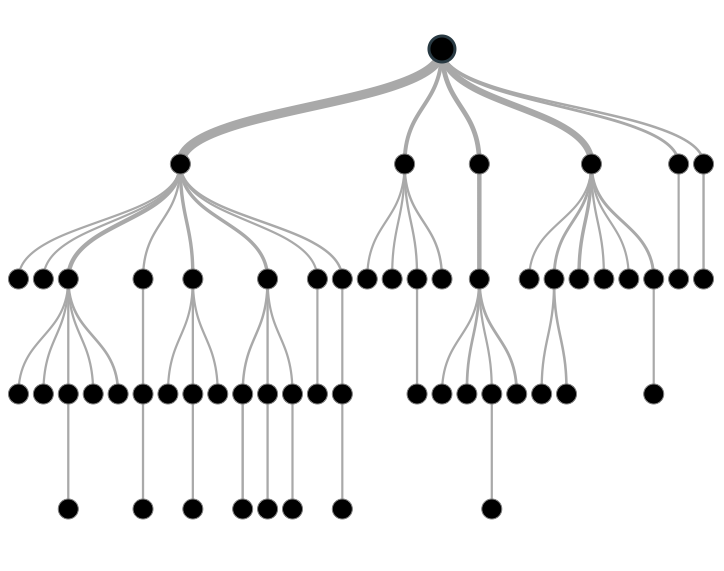
\includegraphics[scale=.4]{figures/dt.png}
	%\flushleft 
	\caption{Visualisering af machine learning beslutningstræ}
	\label{dt}
	%\flushleft
	\textit{Figuren viser en forsimplet visualisering af et vilkårligt beslutningtræ fra en machine learning algoritme.\cite{Saraswat2016}}
\end{figure}

Der findes flere metoder at udføre supervised learning på. En af de første, og stadig populære, er neurale netværk. Her tages der udgangspunkt i et netværk af celler, hvor disse celler får input hvor de i sidste ende summerer deres givne input til en neuron, hvilket kan ses på nedenstående figur. (skal lige have figuren ind)
Fra at cellen får et input til der fås et output fra neuroner, forgår der en proces mellem de to stadier. Processen her kaldes hidden units, der er egentlig det fundamentale og kan næsten sammenlignes med hjernen. Dataene bliver klassificeret undervejs, af de enkelte celler, hvilket betyder at netværket minimeres for fejl, samt at genereliseringsevnen vil blive stærkere. Det gælder om for netværket, at få opbygget et struktur, så den kan forudsige de aspekter den bliver spurgt ind til. \cite{DIKU2010} En af måderne netværket vil blive stærkere igennem tiden er, at den anvender begrebet feedforward netværk, der betyder at når netværket bliver anvendt bliver den trænet, samt også efter den er blevet anvendt. Dette skyldes blandt andet en mekanisme kaldt backprogproganitation. Netværket går ind og sammenligner det output den får ud sammenlignet med det der blev ønsket, og herefter kan der ud fra sammenlignings grundlaget gives feedback til de hidden units og output unitsene. \fxnote{Har lagt kilden op i mendeley og hedder david, shai shalev- kunne ikke lige finde det navn man skulle citerer til} Et eksempel på et neuralt netværk kan ses på \figref{neunet}.

\begin{figure}[H]
	\centering
	\includegraphics[scale=.8]{figures/neunet.png}
	%\flushleft 
	\caption{Neuralt netværk med skjult lag}
	\label{dt}
%	\flushleft
	\textit{På billedet ses et neuralt netværk med skjult lag. Datainput sker i de røde neuroner, beregnes i det skjulte grønne lag, hvorefter det outputtes i den blå neuron.}
\end{figure}

Andre metoder kan også anvendes til at udføre supervised learning. Support Vector Machines (SVM) er en populær algoritme til særligt praktiske problemer. Boosting-algoritmer, som f.eks. AdaBoost er også populære og anvender et princip hvor mange simple klassifikationer samles i en flertalsafstemning, frem for ét beslutningstræ per datapoint.